\begin{tikzpicture}[every node/.style={outer sep=0pt,thick}]

\node (M1) [draw,minimum width=1cm, minimum height=1cm] {$m_1$};
\node (M2) [draw,minimum width=1cm, minimum height=1cm] at (2, 0) {$m_2$};
\node (M3) [draw,minimum width=1cm, minimum height=1cm] at (4, 0) {$m_3$};

% ground for M1 and wheels
\node (ground) [ground,anchor=north,yshift=-0.25cm,minimum width=1.5cm] at (M1.south) {};
\draw (ground.north east) -- (ground.north west);
\draw [thick] (M1.south west) ++ (0.2cm,-0.125cm) circle (0.125cm)  (M1.south east) ++ (-0.2cm,-0.125cm) circle (0.125cm);

% ground for M2 and wheels
\node (ground) [ground,anchor=north,yshift=-0.25cm,minimum width=1.5cm] at (M2.south) {};
\draw (ground.north east) -- (ground.north west);
\draw [thick] (M2.south west) ++ (0.2cm,-0.125cm) circle (0.125cm)  (M2.south east) ++ (-0.2cm,-0.125cm) circle (0.125cm);

% ground for M3 and wheels
\node (ground) [ground,anchor=north,yshift=-0.25cm,minimum width=1.5cm] at (M3.south) {};
\draw (ground.north east) -- (ground.north west);
\draw [thick] (M3.south west) ++ (0.2cm,-0.125cm) circle (0.125cm)  (M3.south east) ++ (-0.2cm,-0.125cm) circle (0.125cm);

\node[ground, rotate=-90, minimum width=2cm] (wall) at (-2, 0) {};
\draw (wall.north east) -- (wall.north west);

\node[ground, rotate=90, minimum width=2cm] (rwall) at (6, 0) {};
\draw (rwall.north east) -- (rwall.north west);

% \draw [spring] (wall.145) -- ($(M1.north west)!(wall.145)!(M1.south west)$);
\draw [spring] (wall.north) -- node[above, yshift=0.25cm] {$k_1$} (M1.west);
\draw [damper] (M1.east) -- node[above, yshift=0.25cm] {$d_1$} (M2.west);
\draw [spring] (M2.east) -- node[above, yshift=0.25cm] {$k_2$} (M3.west);
\draw [damper] (M3.east) -- node[above, yshift=0.25cm] {$d_2$} (rwall.north);

% arrows for directions and things
\draw[thick, dashed] ($(M1.north west)$) -- ($(M1.north west) + (0,1)$);
\draw[thick, dashed] ($(M2.north west)$) -- ($(M2.north west) + (0,1)$);
\draw[thick, dashed] ($(M3.north west)$) -- ($(M3.north west) + (0,1)$);

\draw[ultra thick, -latex] ($(M1.north west) + (0,0.75)$) -- 
    ($(M1.north west) + (1,0.75)$)
    node [midway, below] {$x_1$};
\draw[ultra thick, -latex] ($(M2.north west) + (0,0.75)$) -- 
    ($(M2.north west) + (1,0.75)$)
    node [midway, below] {$x_2$};
\draw[ultra thick, -latex] ($(M3.north west) + (0,0.75)$) -- 
    ($(M3.north west) + (1,0.75)$)
    node [midway, below] {$x_3$};

\draw[ultra thick, -latex]  ($(M1.north west) + (-1,0.75)$) node[above left] {$f(t)$} -- ($(M1.north west) + (0, 0.75)$); 
\end{tikzpicture}

\begin{prob}
    Consider the mechanical system shown in~\cref{fig:trans_system}.
    You can assume that the masses roll on frictionless wheels.
    \begin{figure}[h]
        \centering
        \begin{tikzpicture}[every node/.style={outer sep=0pt,thick}, scale=1]

            \node (M1) [draw,minimum width=1cm, minimum height=1cm] {$m_1$};
            \node (M2) [draw,minimum width=1cm, minimum height=1cm] at (2, 0) {$m_2$};

            % ground for M1 and wheels
            \node (ground) [ground,anchor=north,yshift=-0.25cm,minimum width=1.5cm] at (M1.south) {};
            \draw (ground.north east) -- (ground.north west);
            \draw [thick] (M1.south west) ++ (0.2cm,-0.125cm) circle (0.125cm)  (M1.south east) ++ (-0.2cm,-0.125cm) circle (0.125cm);

            % ground for M2 and wheels
            \node (ground) [ground,anchor=north,yshift=-0.25cm,minimum width=1.5cm] at (M2.south) {};
            \draw (ground.north east) -- (ground.north west);
            \draw [thick] (M2.south west) ++ (0.2cm,-0.125cm) circle (0.125cm)  (M2.south east) ++ (-0.2cm,-0.125cm) circle (0.125cm);

            \node[ground, rotate=-90, minimum width=2cm] (wall) at (-2, 0) {};
            \draw (wall.north east) -- (wall.north west);

            % \draw [spring] (wall.145) -- ($(M1.north west)!(wall.145)!(M1.south west)$);
            \draw [damper] (wall.north) -- node[above, yshift=0.25cm] {$D$} (M1.west);
            \draw [spring] (M1.east) -- node[above, yshift=0.25cm] {$K$} (M2.west);

            % arrows for directions and things
            \draw[thick, dashed] ($(M1.north west)$) -- ($(M1.north west) + (0,1)$);
            \draw[thick, dashed] ($(M2.north west)$) -- ($(M2.north west) + (0,1)$);

            \draw[ultra thick, -latex] ($(M2.north west) + (0,0.75)$) -- 
                ($(M2.north west) + (1,0.75)$)
                node [midway, below] {$x_2$};
            \draw[ultra thick, -latex] ($(M1.north west) + (0,0.75)$) -- 
                ($(M1.north west) + (1,0.75)$)
                node [midway, below] {$x_1$};
            \draw[ultra thick, -latex] (M2.east) -- ($(M2.east) + (1, 0)$) 
                node [right] {$f(t)$}; 
        \end{tikzpicture}
        \caption{Translational Mechanical System~\label{fig:trans_system}}
    \end{figure}

    \begin{subprob}
        \item Find the differential equations of motion for this system.
        \item Defining the state of the system as
            \begin{align*}
                \vecbf{x} = \begin{bmatrix} x_1 & \dot{x}_1 & x_2 & \dot{x}_2 \end{bmatrix}^T ,
            \end{align*}
            find the state equation for this mechanical system.
        \item Find the output equation if the desired output is \( x_2(t) \).
    \end{subprob}
\end{prob}

\clearpage\newpage
\begin{prob}
    Consider the mechanical system in~\cref{fig:triple_mass}.
    Assume that all components have a numerical  value of \( 1 \).
    
    \begin{figure}[h]
        \centering
\begin{tikzpicture}[every node/.style={outer sep=0pt,thick}]

\node (M1) [draw,minimum width=1cm, minimum height=1cm] {$m_1$};
\node (M2) [draw,minimum width=1cm, minimum height=1cm] at (2, 0) {$m_2$};
\node (M3) [draw,minimum width=1cm, minimum height=1cm] at (4, 0) {$m_3$};

% ground for M1 and wheels
\node (ground) [ground,anchor=north,yshift=-0.25cm,minimum width=1.5cm] at (M1.south) {};
\draw (ground.north east) -- (ground.north west);
\draw [thick] (M1.south west) ++ (0.2cm,-0.125cm) circle (0.125cm)  (M1.south east) ++ (-0.2cm,-0.125cm) circle (0.125cm);

% ground for M2 and wheels
\node (ground) [ground,anchor=north,yshift=-0.25cm,minimum width=1.5cm] at (M2.south) {};
\draw (ground.north east) -- (ground.north west);
\draw [thick] (M2.south west) ++ (0.2cm,-0.125cm) circle (0.125cm)  (M2.south east) ++ (-0.2cm,-0.125cm) circle (0.125cm);

% ground for M3 and wheels
\node (ground) [ground,anchor=north,yshift=-0.25cm,minimum width=1.5cm] at (M3.south) {};
\draw (ground.north east) -- (ground.north west);
\draw [thick] (M3.south west) ++ (0.2cm,-0.125cm) circle (0.125cm)  (M3.south east) ++ (-0.2cm,-0.125cm) circle (0.125cm);

\node[ground, rotate=-90, minimum width=2cm] (wall) at (-2, 0) {};
\draw (wall.north east) -- (wall.north west);

\node[ground, rotate=90, minimum width=2cm] (rwall) at (6, 0) {};
\draw (rwall.north east) -- (rwall.north west);

% \draw [spring] (wall.145) -- ($(M1.north west)!(wall.145)!(M1.south west)$);
\draw [spring] (wall.north) -- node[above, yshift=0.25cm] {$k_1$} (M1.west);
\draw [damper] (M1.east) -- node[above, yshift=0.25cm] {$d_1$} (M2.west);
\draw [spring] (M2.east) -- node[above, yshift=0.25cm] {$k_2$} (M3.west);
\draw [damper] (M3.east) -- node[above, yshift=0.25cm] {$d_2$} (rwall.north);

% arrows for directions and things
\draw[thick, dashed] ($(M1.north west)$) -- ($(M1.north west) + (0,1)$);
\draw[thick, dashed] ($(M2.north west)$) -- ($(M2.north west) + (0,1)$);
\draw[thick, dashed] ($(M3.north west)$) -- ($(M3.north west) + (0,1)$);

\draw[ultra thick, -latex] ($(M1.north west) + (0,0.75)$) -- 
    ($(M1.north west) + (1,0.75)$)
    node [midway, below] {$x_1$};
\draw[ultra thick, -latex] ($(M2.north west) + (0,0.75)$) -- 
    ($(M2.north west) + (1,0.75)$)
    node [midway, below] {$x_2$};
\draw[ultra thick, -latex] ($(M3.north west) + (0,0.75)$) -- 
    ($(M3.north west) + (1,0.75)$)
    node [midway, below] {$x_3$};

\draw[ultra thick, -latex]  ($(M1.north west) + (-1,0.75)$) node[above left] {$f(t)$} -- ($(M1.north west) + (0, 0.75)$); 
\end{tikzpicture}
    \caption{Triple Mass system~\label{fig:triple_mass}}
    \end{figure}

    \begin{subprob}
        \item Find the differential equation for the system.
        \item Find the state equation assuming the state is defined as
            \begin{align*}
                \vecbf{x} = \begin{bmatrix} x_1 & \dot{x}_1 & x_2 & \dot{x}_2 & x_3 & \dot{x}_3\end{bmatrix}^T
            \end{align*}

        \item Find the output equation if \( x_3(t)\) is the desired output.
    \end{subprob}
\end{prob}

\begin{prob}
    In this problem we consider the double pendulum on a cart as shown in~\cref{fig:double_pendulum}.
    \begin{figure}[h]
        \centering
        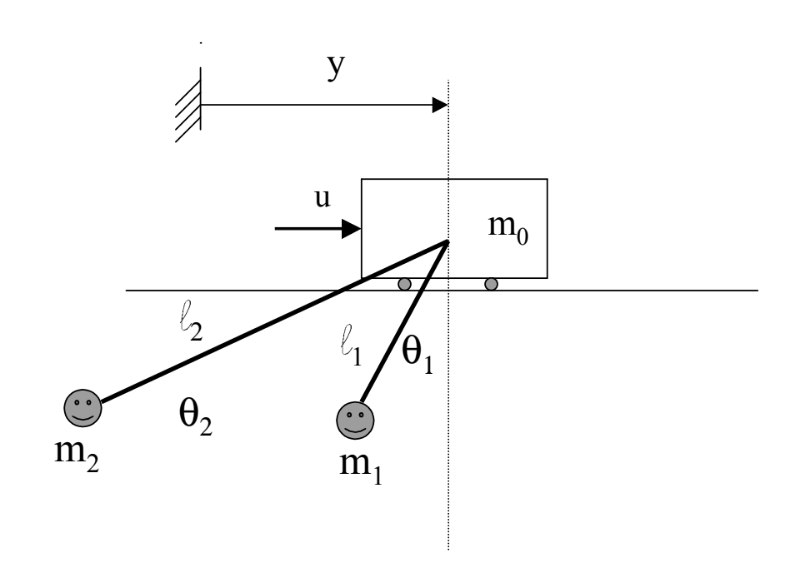
\includegraphics[width=0.5\textwidth]{figures/double_pendulum.png}
        \caption{Double pendulum on a cart}
        \label{fig:double_pendulum}
    \end{figure}
    We will consider the system as an input-ouput system with input \( u \) and output \( y \) as described by
    \begin{align*}
        \parenth{m_0 + m_1 + m_2} \ddot y - m_1 l_1 \cos \theta_1 \ddot \theta_1 - m_2 l_2 \cos \theta_2 \ddot \theta_2 &+ m_1 l_1 \sin \theta_1 \dot \theta_1^2 + m_2 l_2 \sin \theta_2 \dot \theta_2^2 &= u , \\
        -m_1 l_1 \cos \theta_1 \ddot y + m_1 l_1^2 \ddot \theta_1 &+ m_1 l_1 g \sin \theta_1 &= 0 , \\
        - m_2 l_2 \cos \theta_2 \ddot y + m_2 l_2 ^2 \ddot \theta_2 &+ m_2 l_2 g \sin \theta_2 &= 0
    \end{align*}
    \begin{subprob}
    \item For what constant values of \( u \) does the system have equilibrium states?
    \end{subprob}
\end{prob}
